\fancyhead[L]{RF-Positioning System}
\newpage

\section{Introduction}

This document describes the RF-Positioning System, a cost-effective two-axis antenna positioner with a small footprint, intended for characterizing antenna directionality in azimuth and elevation around a fixed centre of rotation. It covers the system's operating principles, its SCPI interface, and the maintenance and service procedures needed to keep it running.

\section{Specifications \& Requirements}

The RF-Positioning System is built to the following specifications \cite{timothy_foley_low-cost_2017, maturo_gmbh_ota_nodate, innco_systems_gmbh_de3600_nodate, microwave_vision_group_light_2025, ets-lindgren_2117_nodate, tdk_rf_solutions_3-dimensional_2024}:
\begin{itemize}
    \item \textbf{Positioning Range:} \SI{360}{\degree} independent rotation in azimuth and elevation
    \item \textbf{Positioning Accuracy:} \SI{1.0}{\degree}
    \item \textbf{DUT Height above Base:} \SI{1.0}{\meter}
    \item \textbf{Base Footprint:} \SI{40}{\centi\meter} x \SI{40}{\centi\meter}
    \item \textbf{Minimum Positioning Speed:} \SI{0.1}{\degree/\second}
    \item \textbf{Maximum Positioning Speed:} \SI{180}{\degree/\second}
    \item \textbf{Payload:} \SI{500}{\gram} 
    \item \textbf{Frequency Range:} \SI{600}{\mega\hertz}~\textendash~\SI{6}{\giga\hertz} 
    \item \textbf{Communication:} USB, Ethernet
    \item \textbf{Power Supply:} \SI{12}{\volt} DC
    \item \textbf{Total Weight:} \SI{\sim 20}{\kilo\gram}
\end{itemize}

\section{Theory of Operation}


\subsection{Mechanical Design}
Most commercial designs opt to only implement elevation rotation on the mast and use a large turntable to provide azimuth rotation. In order to maintain a smaller footprint, while still keeping the centre of mass of the DUT constant during rotation, this design has moved the azimuth rotation to the top of the mast. Figure \ref{fig:mechanical_design} shows how this is achieved using two shafts to transfer the rotation from the motors to the top of the mast. 

In the base unit, both shafts are kept in place by a set of bearings. The stepper motors are coupled to the shafts using a set of timing belts. 

The shaft for the azimuth rotation is mounted off centre and has a gear mounted to the top end, which interfaces with a negative gear on the inside of the head unit. Meanwhile, the elevation shaft is mounted in the centre of the mast aligned with the azimuth axis of rotation. At the top of the shaft, a set of bevel gears is used to transfer the rotation out of the side of the head unit. From there, another timing belt is used to transfer the rotation to the top of the secondary mast, where the DUT is mounted.

The main drawback to this design is that the elevation rotation is coupled to the azimuth rotation. This adds some complexity to the control algorithm, as in order to maintain the elevation angle when the azimuth angle is changed, the elevation motor needs to be moved in sync with the azimuth motor. 

\begin{figure}[h!]
    \centering
    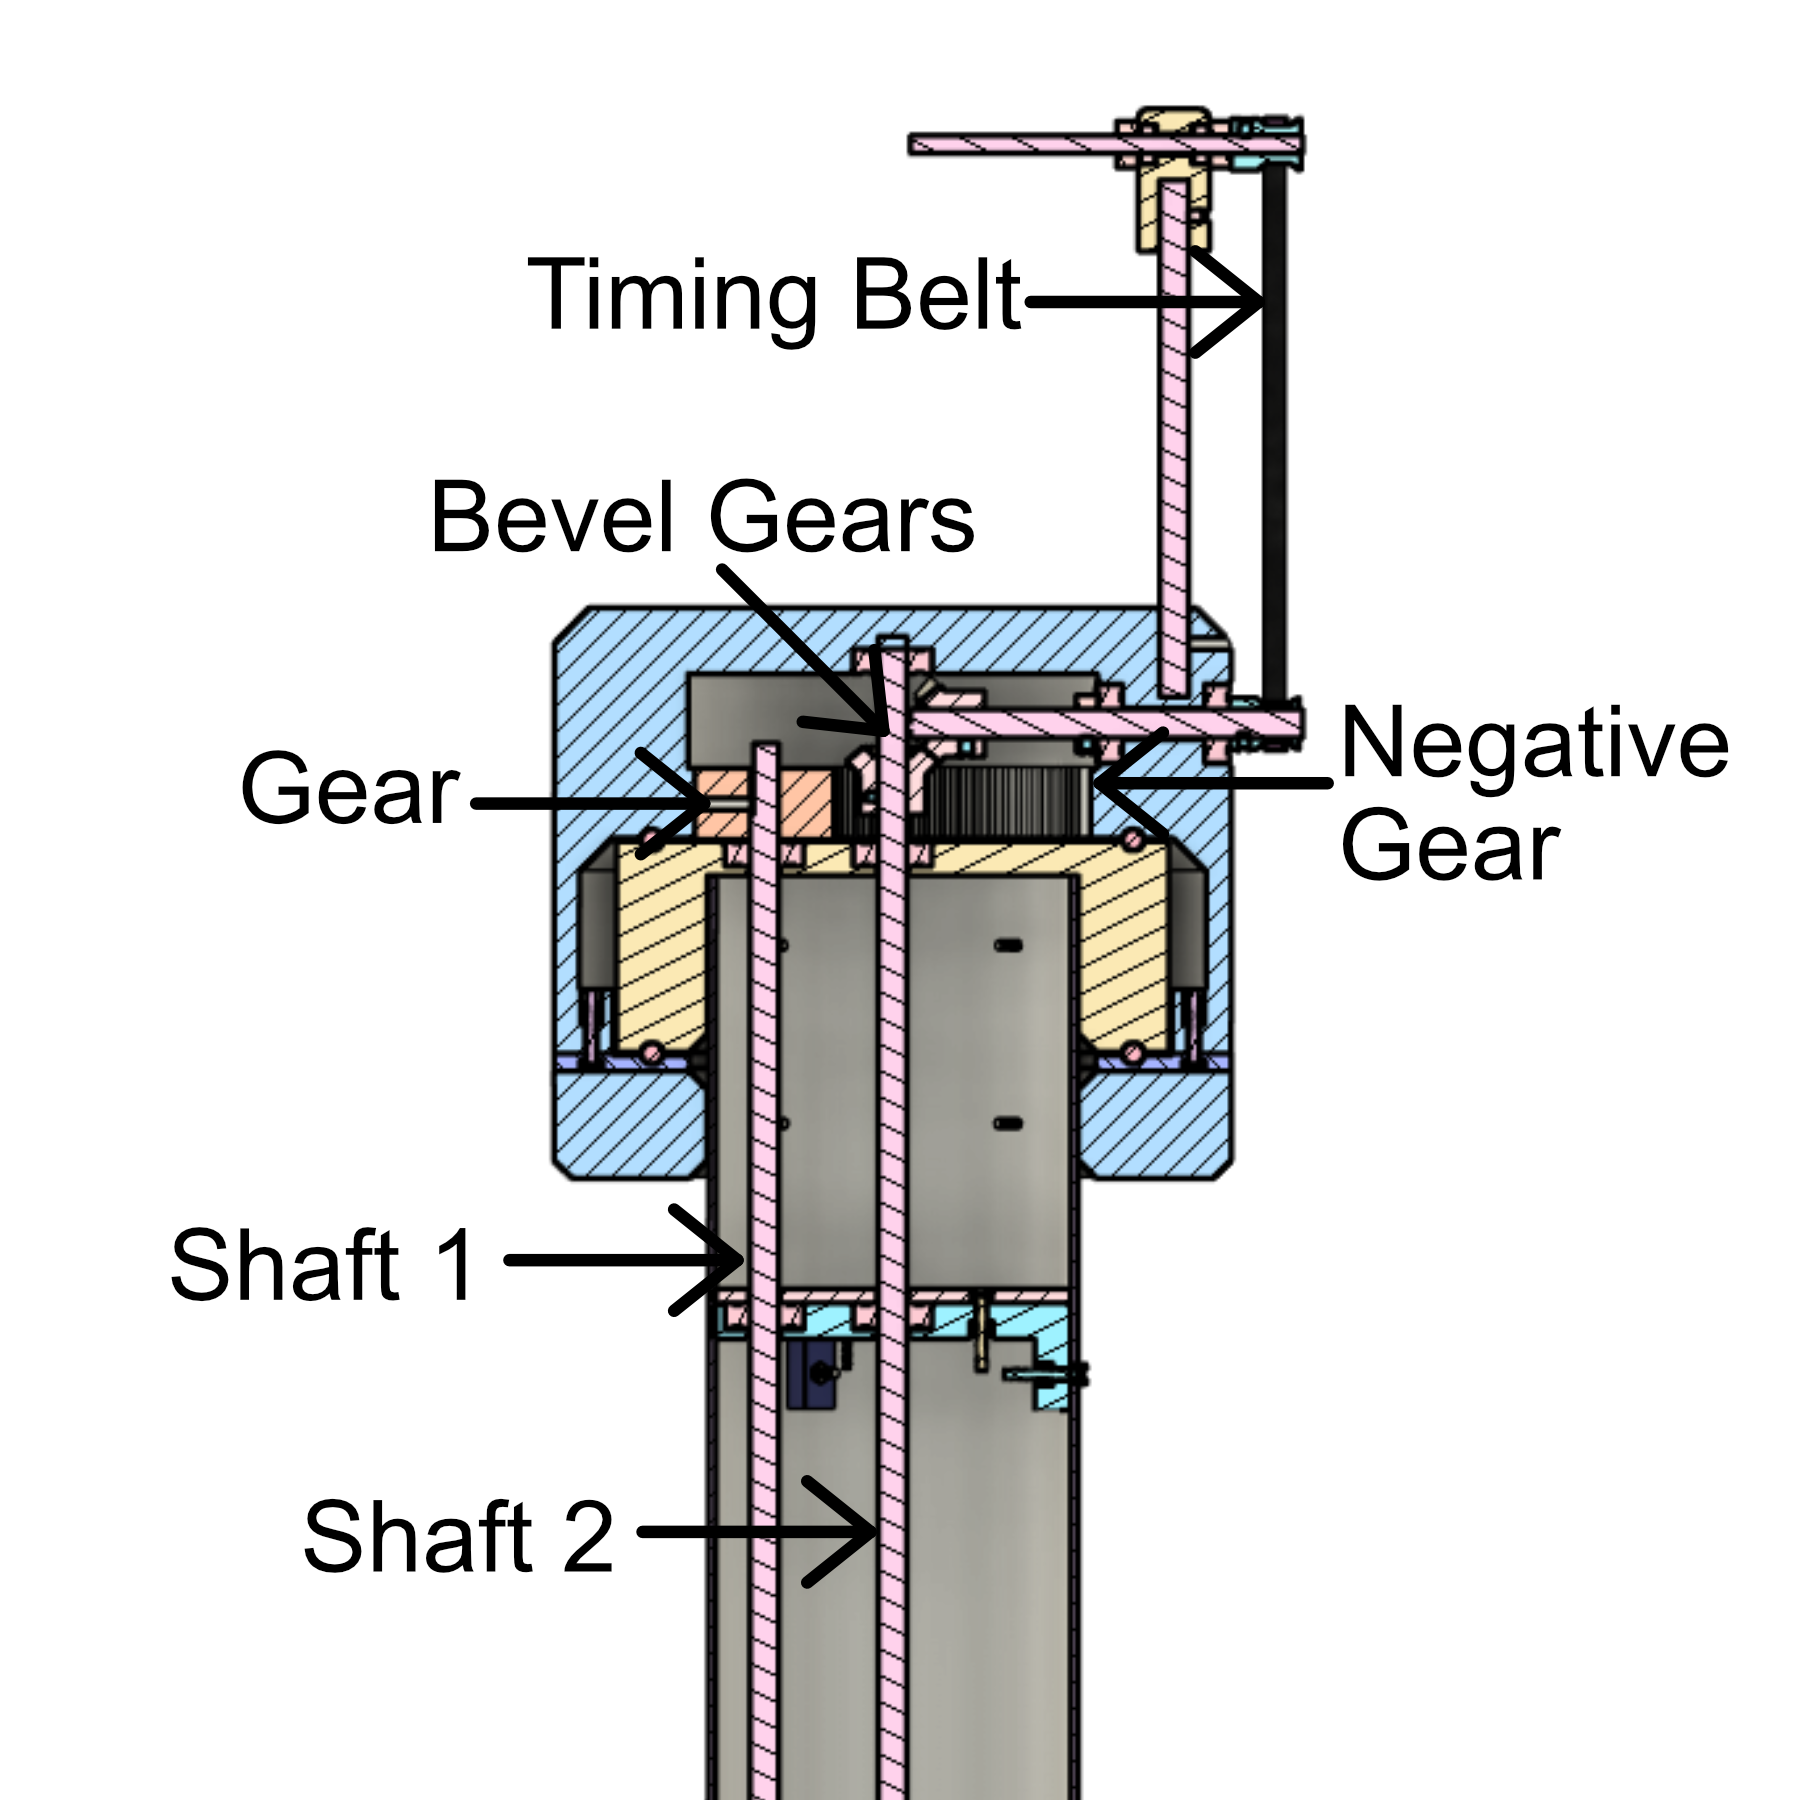
\includegraphics[width=0.8\textwidth]{../assets/LabeledHead.png}
    \caption{Labelled rotation mechanism in the head unit.}
    \label{fig:mechanical_design}
\end{figure}

\subsection{Choice of Materials}
Under the main objective of using only non-conductive materials outside of the base, material choice was driven by the need to balance a low dielectric constant, to minimize interference with RF measurements, with high mechanical strength.

Polylactic Acid (PLA) was chosen for the 3D printed components, which make up most of the head unit, as well as the shaft stabilizers in the pipe. In 2018, Veseleý et al. measured in \cite{vesely_evaluation_2018} that 3D Printed PLA had a dielectric constant $\epsilon_r$ of slightly less than 2.0, for frequencies from 1kHz to 100kHz, with the trend showing a slight decrease for higher frequencies. It should be noted that these values were measured for a frequency range much lower than the RF frequencies used in this project. However, it is assumed that the dielectric constant will not increase significantly for higher frequencies. Additionally, these values were measured for parts with an infill density of \SI{100}{\percent}, while the parts in this project were printed with an infill density of \SI{20}{\percent}. This should significantly reduce the dielectric constant, as \SI{80}{\percent} of the material is replaced with air. Therefore, an $\epsilon_r$ of 2.0 should give a sufficient worst case estimate for the dielectric constant of the 3D printed parts.

For the printed parts fixing the pipe and the motors to the base, a higher strength material was required. As this would be in the shielded base, the dielectric constant is not critical. For this reason, a polyamide with carbon fibre reinforcing particles (PA-CF) was chosen for the additional strength and rigidity. Compared to the PLA, the PA-CF has significantly larger flexural modulus\footnote{Stiffness of the material when bent, a larger value indicates a stiffer material.} (\SI{8.0}{\giga\pascal} vs. \SI{3.2}{\giga\pascal}) as well as a higher charpy impact strength\footnote{The charpy impact strength describes the amount of energy a material can absorb under flexural shock (being struck by a hammer) before breaking.} (\SI{60}{\kilo\joule\per\square\metre} vs. \SI{13}{\kilo\joule\per\square\metre})\cite{formfutura_bv_technical_2023},\cite{prusa_polymers_technical_2022}. It should however be noted, that the conductive carbon fibres in the PA-CF, which provide the additional stiffness, may have a negative effect on the signal integrity, which makes the material unsuitable for use in the RF path.

Another area where material choice was critical, are the fasteners used in the head unit. For the majority of these fasteners, polyamide screws were chosen, as they are commercially available at a low cost. Polyamide typically has a dielectric constant of 3.5 at \SI{1}{\mega\hertz} in dry conditions. However, the material is highly hygroscopic, which means that this value increases up to 7.0 at \SI{50}{\percent} humidity \cite{rolec_gehause-systeme_gmbh_polyamid_pa6_en-_nodate}. This is not ideal, however still significantly better than using metal screws. If there were commercially available screws made from a less hygroscopic material that still fulfil the strength requirements this would be an area where the design could be further improved. For the grub screws used to secure the gears to the shafts, a plastic screw would not provide sufficient strength to keep the gears from slipping on the shaft. For this reason, steel screws with a diameter of \SI{4}{\milli\metre} and a length of \SI{5}{\milli\metre} were chosen. The dimensions here are critical, as the longest side is equivalent to $\lambda/10$ for the maximum frequency of \SI{6}{\giga\hertz} used in this project, which means that it will not significantly interfere with the RF measurements. This is due to the fact that objects smaller than $\lambda/10$ predominantly interact with the RF signals through Rayleigh scattering \cite{nave_blue_nodate}.
																			
\subsection{Motors \& Drivers}
The positioning system uses stepper motors, as these provide accurate positioning at a low cost without needing a closed loop feedback system. The motors are driven using Trinamic TMC2209 stepper motor drivers, which offer a large number of optional features, accessible over their UART interface. One of the features is StallGuard4™ collision detection. As it is not possible to add sensors for a closed loop feedback system in the head unit without running metal wires through the RF path, this feature can give a good indication when a rotational axis has gotten stuck and the stepper motor has lost steps. Another useful feature is the ability to set the current limit for the motor driver, as well as a separate hold current over the UART interface. This allows the system to reduce the current to a minimum when the motors are not moving during measurements, which reduces the radiated emission from the motors \cite{trinamic_motion_control_gmbh__co_kg_tc2209_2016},\cite{trinamic_motion_control_gmbh__co_kg_-015_2015}.

\subsection{Communication}
For communication, the positioning system primarily uses the SCPI (Standard Commands for Programmable Instruments) protocol, hosted over ethernet. The SCPI protocol was chosen, as it is a standardised protocol for programmable instruments and is widely used in the industry. This allows the positioning system to be easily integrated into existing test setups and automated test systems. The connection over ethernet was chosen due to the wide supply of affordable peripherals, from cables and switches to fibre optic converters, should these be required to prevent radiated emissions from the ethernet cable. Additionally, many test chambers will already be equipped with ethernet filters for outgoing connections. The ethernet interface also allows for a simple integration into existing test setups, as most modern computers and test equipment have an ethernet interface.

There is also a backup interface over USB, which is primarily used for configuring the device and for debugging. It is not very practical for use in a RF test chamber, as it would require running a USB cable out of the chamber to a computer, but it allows the user to easily reconfigure the network settings of the device, if the device is not reachable over the network.

For the implementation of the SCPI protocol, the VREKRER SCPI parser library was used \cite{chavez_vrekrervrekrer_scpi_parser_2025}. This allowed for a significant reduction in development time, as the library was able to handle most of the parsing and command handling, so that only a few features such as the error queue and the ethernet interface had to be implemented manually. 

\subsection{Power Supply}
The stepper motors are currently powered from a generic 12V DC power supply. Although the TMC2209 stepper motor drivers are rated for a maximum voltage of 29V, which would provide more torque at higher speeds, the lower voltage was chosen as it limits the rise and fall times of the current in the motor coils. This is desirable, as it reduces the slope, leading to reduced radiated harmonic emissions.

Currently, the ESP32 is powered from the onboard USB port, which is always connected to a computer during the development phase. For the final deployment this would be rather unpractical, so the onboard voltage regulator will be disabled by connecting the "Enable" pin on the ESP32 module to ground. This will allow the use of an external linear regulator to generate the required 3.3V from the 12V supply used for the stepper motors. For this application, a linear regulator is preferred over a switching regulator, as it eliminates a potential source of high frequency interference in the RF test chamber. 

Additionally, several bypass capacitors will be added to the power lines in accordance with the recommendations in the TMC2209 datasheet \cite{trinamic_motion_control_gmbh__co_kg_tc2209_2016}. These will help to ensure a reliable power supply for the stepper motor drivers. They have already been added to the schematic attached to this document.

\subsection{Firmware}
The firmware is written in the PlatformIO Framework and documented using Doxygen \cite{platformio_labs_platformio_nodate}, \cite{van_heesch_doxygen_nodate}. The firmware uses an object oriented approach, with individual classes for each of the core components of the system (stepper motors, SCPI, flash memory, etc.). The full firmware documentation can be found at \url{https://heinekamp.github.io/RF-Positioning-System/index.html}.

\newpage

\section{SCPI Interface}

\subsection{Getting Started}

The positioning system uses SCPI, which is a standardised command set for programmable instruments. SCPI was standardised in 1990 as an extension to the IEEE-488 standard (GPIB Bus). In contrast to the IEEE-488 standard, SCPI does not standardize the physical layer \cite{scpi_consortium_standard_1999}, \cite{noauthor_ieee_1987}. The positioning system accepts SCPI commands over its ethernet interface as well as via UART over the USB interface. It is fully standard compliant with regard to syntax, however not all of the required commands for full standard compliance were implemented due to the simple nature of the device. The following sections will describe how to connect to the device over both interfaces, as well as show a short example script for automating the device with python.

\subsubsection{Connecting over USB}

By default the positioning system is set up to receive serial commands in the following format, enabling compatibility to e.g. the Arduino IDE's Serial Monitor.
\begin{multicols}{2}
\begin{itemize}
    \itemsep0em 
    \item Baudrate: 9600
    \item Data Bits: 8
    \item Stop Bits: 1
    \item Parity: None
    \item Flow Control: None
    \item Termination Character: \texttt{\textbackslash n} (New line)
\end{itemize}
\end{multicols}

\begin{warningbox}
    PUTTY uses a carriage return (\texttt{\textbackslash r}) as the termination character. If you intend to use PUTTY to connect to the device via USB, you will need to change the termination character in the configuration file of the source code and recompile the firmware.
\end{warningbox}

\textbf{Using the Arduino IDE:}

\begin{enumerate}
    \item Install the Arduino IDE from https://www.arduino.cc/en/software/
    \item Connect the positioning system to your computer using the USB port on the ESP32
    \item Select the board from the drop down menu in the upper left 
    \item Open the serial monitor from Tools -> Serial Monitor
    \item Ensure the baud rate is set to 9600 (this should be the default value)
    \item Type *IDN? in the message field and send it using the enter key.
    \item If the positioning system returns a string along the lines of "EMES, RF-Positioning-System, V1.0.0, \#001", a successful serial connection has been established.
\end{enumerate}

\subsubsection{Connecting over Ethernet}
Upon boot, the positioning system will automatically assign itself a static IP address. The default value for this IP address is 192.168.0.55.

If a USB connection has been established, the current IP address may also be queried using the SYSTem:COMMunicate:ETHernet:ADDRess? command. An alternate IP address can also be set using the command SYSTem:COMMunicate:ETHernet:ADDRess <ip address>. Note that a reboot will be required for this change to take effect, a simple means to accomplish this is the *RST command.

A simple method to manually send commands over ethernet is to use the putty terminal emulator~\cite{simon_tatham_download_2025}. For an automated setup using a python script, see section \ref{sec:example_script}. The following steps will show how to connect to the positioning system over ethernet using putty:

\begin{enumerate}
    \item Install putty from \url{https://www.chiark.greenend.org.uk/~sgtatham/putty/latest.html}
    \item Open putty and select the "Raw" connection type under the other section on the session page.
    \item Enter the IP address of the positioning system in the "Host Name (or IP address)" field on the session page.
    \item Enter the port number in the "Port" field on the session page. The default port is 5025, which is the standard port for SCPI communication.
    \item For all other settings, the default values should be sufficient. Open the connection by clicking the "Open" button.
    \item Once the connection is established, you should see a blank terminal window. Type *IDN? in the terminal and press enter.
    \item If the positioning system returns a string along the lines of "EMES, RF-Positioning-System, V1.0.0, \#001", a successful ethernet connection has been established.
    
\end{enumerate}

\subsection{Example Script} \label{sec:example_script}
The following shows a simple example python script to connect to the positioning system over ethernet. It shows how to connect to the device, query the device ID, set some parameters, set some target positions and query the current position. The script uses the PyVISA library~\cite{pyvisa_authors_pyvisa_2025} to connect to the device.

\begin{lstlisting}[language=Python, caption={Example script to connect to the positioning system over ethernet or usb.}, label={lst:example_script}]

import pyvisa
import time

# Connect to the positioning system over Ethernet
rm = pyvisa.ResourceManager()
EthInstrument = rm.open_resource('TCPIP0::192.168.0.55::5025::SOCKET')
EthInstrument.write_termination = '\r\n'
EthInstrument.read_termination = '\n'

# Set a higher timeout, e.g., 10 seconds
EthInstrument.timeout = 10000  # Timeout in milliseconds

print(EthInstrument.query("*IDN?")) # Query and Print the IDN of the instrument

EthInstrument.write("CONFigure:MOTor:SPEED 5000") # Set the motor speed to 5000
EthInstrument.write("CONFigure:MOTor:ACCeleration 5000") # Set the motor acceleration to 5000

EthInstrument.write("CONTRol:ROTation:RELative2 360") # Rotate the motor 360 degrees

while (EthInstrument.query("*OPC?") != "1"):
        time.sleep(0.1) # Wait for the operation to complete

EthInstrument.write("CONFigure:MOTor:ACCeleration 1000") # Set the motor acceleration to 5000

for i in range(36):
    EthInstrument.write("CONTRol:ROTation:RELative2 10") # Rotate the motor 10 degrees
    print(EthInstrument.query("CONTRol:ROTation:ABSolute2?")) # Query the absolute position of the motor
    while (EthInstrument.query("*OPC?") != "1"):
        time.sleep(0.1) # Wait for the operation to complete
    time.sleep(1)

EthInstrument.write("CONFigure:MOTor:SPEED 20000") # Set the motor speed to 20000
EthInstrument.write("CONFigure:MOTor:ACCeleration 5000") # Set the motor acceleration to 5000
EthInstrument.write("CONTRol:ROTation:RELative2 360") # Rotate the motor 360 degrees

EthInstrument.write("CONTRol:ROTation:DIRection2 CCW") # Set the motor direction to counter-clockwise
EthInstrument.write("CONFigure:MOTor:SPEED 5000") # Set the motor speed to 5000
EthInstrument.write("CONTRol:ROTation:RELative2 360") # Rotate the motor 360 degrees

EthInstrument.write("CONTRol:ROTation:DIRection2 CW") # Set the motor direction to clockwise
EthInstrument.write("CONTRol:ROTation:RELative2 360") # Rotate the motor 360 degrees

for i in range(360):
    EthInstrument.write(f"CONTRol:ROTation:ABSolute2 {i}")
    print(EthInstrument.query("CONTRol:ROTation:ABSolute2?")) # Query the absolute position of the motor
    while (EthInstrument.query("*OPC?") != "1"):
        time.sleep(0.1) # Wait for the operation to complete

\end{lstlisting}


\newpage

\subsection{Command Reference} \label{sec:command_reference}

\subsubsection{Command Overview}


\begin{itemize}[label={}]
    \item \textbf{*IDN?}
    \vspace{-0.25em}
    \item \textbf{*RST}
    \vspace{-0.25em}
    \item \textbf{*OPC?}
    \vspace{-0.25em}
    \item \textbf{SYSTem}
    \vspace{-0.25em}
    \begin{itemize}[label={}]
        \item \texttt{:ERRor?}
        \item \texttt{:HELP:HEADers?}
        \item \texttt{:HELP:SYNTax?}
        \item \texttt{:VERSion?}
        \item \texttt{:DEBUG?}
        \item \texttt{:PRESet}
        \item \texttt{:COMMunicate:ETHernet}
        \begin{itemize}[label={}]
            \item \texttt{:PORT}
            \item \texttt{:PORT?}
            \item \texttt{:ADDRess}
            \item \texttt{:ADDRess?}
            \item \texttt{:MAC}
            \item \texttt{:MAC?}
            \item \texttt{:DGATeway?}
            \item \texttt{:RESET}
        \end{itemize}
    \end{itemize}
    \vspace{-0.25em}
    \item \textbf{CONTRol:ROTation}
    \vspace{-0.25em}
    \begin{itemize}[label={}]
        \item \texttt{:STEP\#}
        \item \texttt{:PERPetual\#}
        \item \texttt{:DIRection\#}
        \item \texttt{:DIRection\#?}
        \item \texttt{:RELative\#}
        \item \texttt{:ABSolute\#}
        \item \texttt{:ABSolute\#?}
    \end{itemize}
    \vspace{-0.25em}
    \item \textbf{CONFigure:MOTor}
    \vspace{-0.25em}
    \begin{itemize}[label={}]
        \item \texttt{:RMScurrent}
        \item \texttt{:RMScurrent?}
        \item \texttt{:HOLDcurrent}
        \item \texttt{:HOLDcurrent?}
        \item \texttt{:MICROsteps}
        \item \texttt{:MICROsteps?}
        \item \texttt{:SPEED}
        \item \texttt{:SPEED?}
        \item \texttt{:ACCELeration}
        \item \texttt{:ACCELeration?}
        \item \texttt{:STATus?}
    \end{itemize}
    \vspace{-0.25em}
    \item \textbf{DIAGnostic}
    \vspace{-0.25em}
    \begin{itemize}[label={}]
        \item \texttt{:SESSion:LIST?}
        \item \texttt{:SESSion:LOG?}
        \item \texttt{:SOCKet:LIST?}
        \item \texttt{:SYSTem?}
    \end{itemize}
\end{itemize}

\subsubsection{IEEE 488 Mandated Commands}
\textbf{*IDN?} \\
This command returns the device identification string. The string is formatted as follows: <manufacturer>, <model>, V<version>, \#<serial number>. For example, the device returns "EMES, RF-Positioning-System, V1.0.0, \#001".

\textbf{*RST} \\
This command initiates a full reboot on the controller. This will also reset the error queue and set the current position to 0° for both axes. \\
NOTE: This command does not reset the device configuration to its default values. For that please see SYSTem:PRESet.

\textbf{*OPC?} \\
This command returns 1 when all commands sent before this command have been executed. For example, this command can be used to ensure that the positioning system has reached the target position before any measurements are started.

\subsubsection{System Commands} \label{sec:system_commands}
\textbf{SYSTem:ERRor?} \\
This command returns the oldest error in the error queue. The error is returned as a string in the format "<error code>, <error message>". The error queue is a FIFO queue, meaning that the oldest error will be returned first. If there are no errors in the queue, this command will return "0, No Error". \\
NOTE: The error queue has a limited size. If the queue is full, new errors will be ignored and the SYSTem:ERRor? command will return "-350, "Queue overflow". After this the errors already in the queue can be read as normal, however the user should be aware that the most recent errors were not recorded.

\textbf{SYSTem:HELP:HEADers?} \\
This command returns a list of all available SCPI commands.

\textbf{SYSTem:HELP:SYNTax?} \\
This command returns detailed syntax help for a single command header, given as a parameter, e.g. \texttt{SYSTem:HELP:SYNTax? *IDN?}. The header must be given exactly as printed by \texttt{SYSTem:HELP:HEADers?} (matching is case-insensitive, and surrounding quotes are stripped if present). If the header is not recognized, the command returns "UNKNOWN" and queues an error.

\textbf{SYSTem:VERSion?} \\
This command returns the version of the firmware running on the positioning system.

\textbf{SYSTem:DEBUG?} \\
This command returns the debug information from the VREKRER SCPI parser library \cite{chavez_vrekrervrekrer_scpi_parser_2025}. This can be used to debug issues with the SCPI commands sent to the positioning system.

\textbf{SYSTem:PRESet} \\
This command resets the device configuration to the default values stored in the firmware. These can be adjusted by editing the configuration.h file in the source code.

\textbf{SYSTem:COMMunicate:ETHernet:PORT} \\
This command sets the port for the ethernet interface. The default value is 5025, which is the standard port for SCPI communication. \\
NOTE: A full reboot of the controller is required for this change to take effect. A simple means to accomplish this is the *RST command.

\textbf{SYSTem:COMMunicate:ETHernet:PORT?} \\
This command returns the current port for the ethernet interface.

\textbf{SYSTem:COMMunicate:ETHernet:ADDRess} \\
This command sets the IP address for the ethernet interface. The required format is SYSTem:COMMunicate:ETHernet:ADDRess XXX.XXX.XXX.XXX, where XXX is a integer value between 0 and 255. \\
NOTE: A full reboot of the controller is required for this change to take effect. A simple means to accomplish this is the *RST command.

\textbf{SYSTem:COMMunicate:ETHernet:ADDRess?} \\
This command returns the current IP address for the ethernet interface.

\textbf{SYSTem:COMMunicate:ETHernet:MAC} \\
This command sets the MAC address for the ethernet interface. The correct format would be SYSTem:COMMunicate:ETHernet:MAC XX:XX:XX:XX:XX:XX, where XX is a two digit hexadecimal number. \\
NOTE: A full reboot of the controller is required for this change to take effect. A simple means to accomplish this is the *RST command.

\textbf{SYSTem:COMMunicate:ETHernet:MAC?} \\
This command returns the current MAC address for the ethernet interface.

\textbf{SYSTem:COMMunicate:ETHernet:DGATeway?} \\
This command returns the configured default gateway for the ethernet interface as a dotted-quad IPv4 address. \\
NOTE: There is currently no corresponding setter command; the gateway is derived automatically and cannot be set directly over SCPI.

\textbf{SYSTem:COMMunicate:ETHernet:RESET} \\
This command resets the W5500 Ethernet module and re-initializes the network stack: it toggles the module's hardware reset pin, re-reads the IP and MAC address from flash, and restarts the SCPI listener. \\
NOTE: This drops all currently tracked SCPI sessions, including the one issuing this command.

\subsubsection{Rotation Control Commands}

The commands in the following section are used to control both rotation axes of the positioning system. The numeric suffix \# in the command names is used to indicate which axis the command applies to. For the azimuth axis the suffix should be set to 1, while for the elevation axis it should be set to 2. For example, the command to step the azimuth axis would be \texttt{CONTRol:ROTation:STEP1} and for the elevation axis it would be \texttt{CONTRol:ROTation:STEP2}.
\vspace{1em}

\textbf{CONTRol:ROTation:STEP\#} \\
This command jogs the specified axis exactly one full mechanical revolution at a fixed speed, with no acceleration ramp. It does not update the axis's tracked absolute position. This command is intended for testing and troubleshooting the motion system, not for normal operation.

\textbf{CONTRol:ROTation:PERPetual\#} \\
This command runs the specified axis continuously at a fixed speed. It does not return a response, and blocks all further command processing on both the Serial and Ethernet interfaces until the device is reset or power-cycled. \\
NOTE: This command is intended for testing and troubleshooting the motion system, not for normal operation.

\textbf{CONTRol:ROTation:DIRection\#} \\
This command sets the direction of rotation for the specified axis. The command takes a single argument, which can be either "CW" for clockwise or "CCW" for counter-clockwise. For example, to set the azimuth axis to rotate clockwise, the command would be \texttt{CONTRol:ROTation:DIRection1 CW}.

\textbf{CONTRol:ROTation:DIRection\#?} \\
This command returns the current direction of rotation for the specified axis. The return value will be either "CW" for clockwise or "CCW" for counter-clockwise.

\textbf{CONTRol:ROTation:RELative\#} \\
This command sets the target position for the specified axis relative to the current position. The command takes a single argument, which is the angle in degrees to move the axis. For example, to move the azimuth axis by 10 degrees, the command would be \texttt{CONTRol:ROTation:RELative1 10}.

\textbf{CONTRol:ROTation:ABSolute\#} \\
This command sets the target position for the specified axis as an absolute angle. The command takes a single argument, which is the angle in degrees to move the axis. For example, to move the azimuth axis to 90 degrees, the command would be \texttt{CONTRol:ROTation:ABSolute1 90}.

\textbf{CONTRol:ROTation:ABSolute\#?} \\
This command returns the current position of the specified axis in degrees as an absolute angle with respect to the zero position. The zero position is defined as the position when the system was last reset using the *RST command.

\subsubsection{Motor Configuration Commands}

The commands in the following section are used to configure the stepper motors used in the positioning system. They use the same numeric suffix system as the rotation control commands. In adition all of the parameters are live adjustable, meaning that the changes will take effect immediately without the need to reboot the controller.

\textbf{CONFigure:MOTor:RMScurrent} \\
This command sets the RMS current for the specified axis. The command takes a single argument, which is the current in milliamps. For example, to set the azimuth axis to \SI{1000}{\milli\ampere}, the command would be \texttt{CONFigure:MOTor:RMScurrent1 1000}.

\textbf{CONFigure:MOTor:RMScurrent?} \\
This command returns the current RMS current for the specified axis in milliamps.

\textbf{CONFigure:MOTor:HOLDcurrent} \\
This command sets the hold current for the specified axis. The command takes a single argument, which is a value between 0 and 32. The hold current will be set to a fraction over 32 of the RMS current set by the \texttt{CONFigure:MOTor:RMScurrent\#} command. For example, to set the azimuth axis to 50\% of the RMS current, the command would be \texttt{CONFigure:MOTor:HOLDcurrent1 16}.

\textbf{CONFigure:MOTor:HOLDcurrent?} \\
This command returns the current hold current for the specified axis as a value between 0 and 32. The hold current is represented by a fraction over 32 of the RMS current set by the \texttt{CONFigure:MOTor:RMScurrent\#} command.

\textbf{CONFigure:MOTor:MICROsteps} \\
This command sets the number of microsteps for the specified axis. Increasing this value will reduce in a better positioning accuracy, but comes at the cost of reducing the available torque. The command takes a single argument, which is the number of microsteps per step. The valid values are 1, 2, 4, 8, 16, 32, 64 and 128. For example, to set the azimuth axis to 16 microsteps per step, the command would be \texttt{CONFigure:MOTor:MICROsteps1 16}.

\textbf{CONFigure:MOTor:MICROsteps?} \\
This command returns the current number of microsteps set for the specified axis. 

\textbf{CONFigure:MOTor:SPEED} \\
This command sets the speed for the specified axis. The command takes a single argument, which is the speed in degrees per second. For example, to set the azimuth axis to 90 degrees per second, the command would be \texttt{CONFigure:MOTor:SPEED1 90}.

\textbf{CONFigure:MOTor:SPEED?} \\
This command returns the current speed set for the specified axis in degrees per second.

\textbf{CONFigure:MOTor:ACCELeration} \\
This command sets the acceleration for the specified axis. The command takes a single argument, which is the acceleration in degrees per second squared. For example, to set the azimuth axis to 10 degrees per second squared, the command would be \texttt{CONFigure:MOTor:ACCELeration1 10}.

\textbf{CONFigure:MOTor:ACCELeration?} \\
This command returns the current acceleration set for the specified axis in degrees per second squared.

\textbf{CONFigure:MOTor:STATus?} \\
This command returns the raw TMC2209 driver status registers for both axes, as two lines: "Motor 1 Status: <binary>" and "Motor 2 Status: <binary>". These are the raw DRV\_STATUS-style status bits from the driver IC, intended for diagnostic use.

\subsubsection{Diagnostic Commands}

The commands in this section are primarily intended for diagnosing communication issues, such as a client that is unable to establish or maintain a connection to the positioning system.

\textbf{DIAGnostic:SESSion:LIST?} \\
This command lists the currently active SCPI sessions over ethernet. It returns "\#SESSIONS <n>" followed by one CSV line per active session, giving its index, classification (SCPI/PING), TCP state, remote IP, remote port, local port, age, idle time, and received/transmitted byte counts.

\textbf{DIAGnostic:SESSion:LOG?} \\
This command lists recent SCPI session closures. It returns "\#CLOSES <n>" followed by one CSV line per closure (oldest first, up to the last 16), giving the time since it closed, the remote IP:port, the closure reason (EVICTED\_BY\_NEW/CLIENT\_FIN/RST/OTHER), session duration, idle time at close, and received/transmitted byte counts.

\textbf{DIAGnostic:SOCKet:LIST?} \\
This command returns the raw state of all 8 hardware sockets on the W5500 ethernet module, as "\#SOCKETS 8" followed by one CSV line per socket, giving its index, TCP state, and whether it is currently tracked as a SCPI session.

\textbf{DIAGnostic:SYSTem?} \\
This command returns system and reset health diagnostics as comma-separated key=value pairs: uptime in seconds, free heap, minimum free heap seen, the reason for the last reset, the boot count, the number of ethernet link flaps, and the number of ethernet re-initializations.

\subsubsection{Error Codes}
In compliance with the SCPI standard, the positioning system implements an error queue. This will return a error code along with a message for any error that has occurred. As described in Section \ref{sec:system_commands}, the error queue can be queried using the command \texttt{SYSTem:ERRor?}. The error queue is a FIFO queue, meaning that the oldest error will be returned first. An overview of the implemented error codes is shown in Table \ref{tab:error_codes}.

\begin{table}[h!]
\centering
\begin{tabularx}{\textwidth}{|c|X|}
\hline
\textbf{Error Code} & \textbf{Description} \\ \hline
0 & No Error \\ \hline
-350 & Queue overflow \\ \hline
131 & Invalid Suffix \\ \hline
220 & Invalid parameter value \\ \hline
224 & Illegal parameter value \\ \hline
\end{tabularx}
\caption{Error Codes and Descriptions}
\label{tab:error_codes}
\end{table}

\newpage

\section{Service}
\subsection{Maintenance}

\subsubsection{Belt Tension}

For checking the belt tension, the Gates Carbon Drive app \cite{gates_tools_nodate} will be used. It uses the devices microphone to measure the resonant frequency of the belt when plucked. The target frequencies were calculated based on the type and length of the belt and are noted in the corresponding assembly steps below \cite{zoltan_benchtop_2019}. 

\assemblystep{1 Motor Belts}{../assets/assembly/1-belt-tension.png}{\hexkey{2.5mm} \smartphone{}}{
  \begin{itemize}[left=0pt, labelsep=4pt, itemsep=0pt]
    \partitem{part1}{Loosen the four M3x8 screws on each motor using a 2.5mm hex key.}
    \partitem{part2}{Move the motor back and forth to adjust the belt tension. }
    \partitem{part3}{Retighten the screws once the correct belt tenstion is set.}
  \end{itemize}
  \vspace{-1em}
  \begin{notebox}
    The upper belt should be tensioned to \SI{190}{\Hz} and the lower belt to \SI{228}{\Hz}~\cite{zoltan_benchtop_2019}.\\
  \end{notebox}
}
\enlargethispage{2\baselineskip}
\vspace{-\baselineskip}

\assemblystep{2 Top Belt}{../assets/assembly/2-top-belt-tension.png}{\hexkey{2.0mm} \smartphone{}}{
  \begin{itemize}[left=0pt, labelsep=4pt, itemsep=0pt]
    \partitem{part1}{Loosen the M4x5  grub screw using a 2.0mm hex key.}
    \partitem{part2}{Move the bearing holder up and down to adjust the belt tension. }
    \partitem{part3}{Optionally this grub screw can also be loosend to move the entire shaft}
    \partitem{part4}{Retighten the screws once the correct belt tenstion is set.}
  \end{itemize}
  \vspace{-1em}
  \begin{notebox}
    The belt should be tensioned to \SI{159}{\Hz}~\cite{zoltan_benchtop_2019}.
  \end{notebox}
}

\subsection{Component Replacement}

The following section describes how to disassemble the positioning system in order to replace components. To reassemble the system, the steps should be followed in reverse order.

\subsubsection{Stepper Motors}

\assemblystep{1 Stepper Motor}{../assets/assembly/1-remove-motor.png}{\hexkey{2.5mm} }{
    \begin{itemize}[left=0pt, labelsep=4pt, itemsep=0pt]
        \partitem{part1}{Remove the four M3x8 (HW~10) screws on each motor using a 2.5mm hex key.}
        \partitem{part2}{Move the motor towards the main tower to free it from the timing belt.}
      \end{itemize}
}

\assemblystep{2 Timing Pulley \& Wire}{../assets/assembly/2-pulley-wire.png}{\hexkey{2.0mm} }{
  \begin{itemize}[left=0pt, labelsep=4pt, itemsep=0pt]
    \partitem{part1}{Remove the two M4x5 grub screws (HW~9) on each pulley using a 2.0mm hex key.}
    \partitem{part2}{Pull the timing pulley (HW~15) of the shaft.}
    \partitem{part3}{Remove the wire from the motor.}
  \end{itemize}
  \begin{warningbox}
    When reinstalling the timing pulley, ensure that one grub screw is aligned with the flat side of the motor shaft.\\
  \end{warningbox}
}

\assemblystep{3 Motor Mount}{../assets/assembly/3-motor-mount.png}{\torx{T10} }{
  \begin{itemize}[left=0pt, labelsep=4pt, itemsep=0pt]
    \partitem{part1}{Remove the six 3x30mm universal screws (HW~13) using a T10 torx screwdriver. The motor mount can now be removed from the base plate.}
    
  \end{itemize}
}

\subsubsection{Upper mast}
\assemblystep{1 Timing Belt}{../assets/assembly/1-timing-belt.png}{\hexkey{2.0mm} }{
  \begin{itemize}[left=0pt, labelsep=4pt, itemsep=0pt]
    \partitem{part1}{Remove the two M4x5 grub screws (HW~9) using a 2.0mm hex key.}
    \partitem{part2}{Push the bearing holder down towards the shaft and the shaft down into the head unit to relieve the tension on the timing belt.}
    \partitem{part3}{The timing belt (HW~18) can now be removed.}
  \end{itemize}
}

\assemblystep{2 Upper Axle}{../assets/assembly/2-upper-axle.png}{\hexkey{2.0mm} }{
  \begin{itemize}[left=0pt, labelsep=4pt, itemsep=0pt]
    \partitem{part1}{Remove the three M4x5 grub screws (HW~9) from the locking rings and the timing puley using a 2.0mm hex key.}
    \partitem{part2}{The axle (SHAFT4) can now be slid out of the bearing holder, releasing the timing pulley (3D~8) and the locking rings (3D~5).}
  \end{itemize}
  \begin{warningbox}
    When reinstalling the axle, ensure that the timing pulley is aligned with the flat side of the axle.
  \end{warningbox}
}

\assemblystep{3 Bearing Holder \& Shaft}{../assets/assembly/3-bearing-holder-shaft.png}{}{
  \begin{itemize}[left=0pt, labelsep=4pt, itemsep=0pt]
    \partitem{part1}{As the grub screws were already removed in step 1, the bearing holder (3D~7) can now be pulled off the shaft.}
    \partitem{part2}{Following this, the shaft (SHAFT3) can be pulled out of the head unit.}

  \end{itemize}
}

\assemblystep{4 Bearings}{../assets/assembly/4-bearings.png}{\flathead{}}{
  \begin{itemize}[left=0pt, labelsep=4pt, itemsep=0pt]
    \partitem{part1}{Finally, the bearings (HW~3) can be pulled out of the bearing holder. The easiest way to do this is to carefully use a small flathead screwdriver to pry them out.}
  \end{itemize}
  \begin{notebox}
    If the bearings come apart during removal, they can be reassembled by reinserting the bearing balls into the outer ring and then pressing the inner ring back in.
  \end{notebox}
}

\subsubsection{Head Unit}
\assemblystep{1 Lower Head Alignment}{../assets/assembly/1-aligment-ring.png}{\flathead{}}{
  \begin{itemize}[left=0pt, labelsep=4pt, itemsep=0pt]
    \partitem{part1}{Unscrew the four M3x20 screws (HW~7) holding the head alignment ring (3D~4) in place.}
    \partitem{part2}{Lower the head alignment ring until it sits on the mounting screws for the shaft stabilizer.}
  \end{itemize}
  \begin{notebox}
    These screws must only be unscrewed far enough to allow the head alignment ring to be lowered. This way they will still hold the nuts on the inside of the alignment ring in place.
  \end{notebox}
}
\assemblystep{2 Head Bottom Plate}{../assets/assembly/2-head-bottom.png}{\flathead{}}{
  \vspace{-1.5em}
  \begin{itemize}[left=0pt, labelsep=4pt, itemsep=0pt]
    \partitem{part1}{Remove the 10 M3x20 screws (HW~7) holding the head bottom plate (3D~2) in place.}
    \partitem{part2}{Lower the head bottom plate until it sits on the head alignment ring.}
  \end{itemize}
  \vspace{-2.2em}
  \begin{warningbox}
    There are 70 loose bearing balls (HW~4), which sit in a groove ontop of the head bottom plate. It is recommended to unscrew the screws evenly to ensure the plate stays perpendicular to the shaft. Once the plate is lowered far enough, the bearing balls can be carefully removed.
  \end{warningbox}
}
\assemblystep{3 Head Top Assembly}{../assets/assembly/3-head-top.png}{}{
  \vspace{-1.5em}
  \begin{itemize}[left=0pt, labelsep=4pt, itemsep=0pt]
    \partitem{part1}{At this point the remaining top assembly can be pulled up and off the positioning system.}
  \end{itemize}
  \vspace{-1em}
  \begin{warningbox}
    Once again, this will expose 70 loose bearing balls (HW~4), which sit under the top asseembly.
  \end{warningbox}
  \begin{notebox}
    During reassembly this is a good point to verify that the bevel gears are engaging correctly. 
  \end{notebox}
}

\assemblystep{4 Nuts}{../assets/assembly/6-top-nuts.png}{\hexkey{2.5mm}}{
  \begin{itemize}[left=0pt, labelsep=4pt, itemsep=0pt]
    \partitem{part1}{Remove the 20 M3 nuts (HW~11) from the pockets in the head unit.}
  \end{itemize}
    \begin{notebox}
        One of the previously removed M3x20 screws can be used to push the nuts out of the pockets. During reassembly, the nuts can be pulled back into the pockets by sticking the screws though the hole and threading the nuts onto the tip of the screw.
    \end{notebox}
}


\assemblystep{5 Shaft}{../assets/assembly/4-top-shaft.png}{\hexkey{2.0mm}}{
  \vspace{-1.5em}
  \begin{itemize}[left=0pt, labelsep=4pt, itemsep=0pt]
    \partitem{part1}{Remove the two M4x5 grub screws (HW~9) from the locking ring (3D~6) and the bevel gear (HW~1) using a 2.0mm hex key.}
    \partitem{part2}{The shaft (SHAFT3) can now be pulled out of the head unit, thereby releasing the locking ring and the bevel gear.}
    \partitem{part3}{Remove the last grub screw (HW~9) to release the timing pulley (3D~9) from the shaft.}
  \end{itemize}
  \vspace{-1em}
}

\assemblystep{6 Bearings}{../assets/assembly/5-bearings.png}{\flathead{}}{
  \vspace{-1.5em}
  \begin{itemize}[left=0pt, labelsep=4pt, itemsep=0pt]
    \partitem{part1}{Remove the three bearings (HW~2) from the head unit. The easiest way to do this is to carefully use a small flathead screwdriver to pry them out.}
  \end{itemize}
    \begin{notebox}
        If the bearings come apart during removal, they can be reassembled by reinserting the bearing balls into the outer ring and then pressing the inner ring back in.
    \end{notebox}
  \vspace{-1em}
}

\subsubsection{Head Base}
\assemblystep{1 Gears}{../assets/assembly/1-gears.png}{\hexkey{2.0mm}}{
  \begin{itemize}[left=0pt, labelsep=4pt, itemsep=0pt]
    \partitem{part1}{Remove the two M4x5 grub screws (HW~9) from the gears using a 2.0mm hex key.}
    \partitem{part2}{The bevel gear (HW~1) and spur gear (3D~10) can now be pulled off the shaft.}
  \end{itemize}
  \begin{notebox}
    During reassembly, ensure that the grub screws are aligned with the flat side of the shaft.
    
    The bevel gear should be mounted \SI{8}{\milli\meter} above the bearing.
  \end{notebox}
}

\assemblystep{2 Head Base}{../assets/assembly/2-top-base.png}{\hexkey{2.5mm}}{
  \begin{itemize}[left=0pt, labelsep=4pt, itemsep=0pt]
    \partitem{part1}{Remove the four M3x20mm screws (HW~7) from the head base using a 2.5mm hex key.}
    \partitem{part2}{The head base assembly (3D~3) cam now be pulled off the top of the mast.}
  \end{itemize}
}

\assemblystep{3 Nuts}{../assets/assembly/3-top-nuts.png}{}{
  \begin{itemize}[left=0pt, labelsep=4pt, itemsep=0pt]
    \partitem{part1}{Remove the 8 M3 nuts (HW~11) from the pockets in the head base.}
  \end{itemize}
}

\assemblystep{4 Bearings}{../assets/assembly/4-top-bearings.png}{\flathead{}}{
  \begin{itemize}[left=0pt, labelsep=4pt, itemsep=0pt]
    \partitem{part1}{Remove the two bearings (HW~2) from the head base. The easiest way to do this is to carefully use a small flathead screwdriver to pry them out.}
  \end{itemize}
  \begin{notebox}
    If the bearings come apart during removal, they can be reassembled by reinserting the bearing balls into the outer ring and then pressing the inner ring back in.
  \end{notebox}
}

\assemblystep{5 Alignment Ring}{../assets/assembly/5-alignment-ring.png}{\hexkey{2.5mm}}{
  \begin{itemize}[left=0pt, labelsep=4pt, itemsep=0pt]
    \partitem{part1}{Now that the head base is removed, the head alignment ring (3D~4) can be pulled off the top of the mast.}
    \partitem{part2}{Once it is removed, there are eight M3 nuts (HW~11) on the inside of the screw holes, which can be removed as described in step 3.}
  \end{itemize}
}

\subsubsection{Base Assembly}
\assemblystep{1 Mast}{../assets/assembly/1-base-mast.png}{\hexkey{2.5mm}}{
  \begin{itemize}[left=0pt, labelsep=4pt, itemsep=0pt]
    \partitem{part1}{Remove the four M3x20mm screws (HW~8) that are securing the mast to the base using a 2.5mm hex key.}
    \partitem{part2}{At this point the mast can be pulled out of the base assembly.}
  \end{itemize}
}

\assemblystep{2 Base Screws}{../assets/assembly/2-base-screws.png}{\torx{T10}}{
  \begin{itemize}[left=0pt, labelsep=4pt, itemsep=0pt]
    \partitem{part1}{Remove the eight 3x30mm universal screws (HW~13) that are securing the pipe mount (3D~14) to the base plate.}
    \partitem{part2}{The pipe mount can now be removed from the base plate.}
  \end{itemize}
}

\assemblystep{3 Bearings \& Nuts}{../assets/assembly/3-pipe-mount.png}{\flathead{}}{
  \begin{itemize}[left=0pt, labelsep=4pt, itemsep=0pt]
    \partitem{part1}{Remove the eight M3 nuts (HW~12) from the pipe mount (3D~14). These nuts are located in the pockets on the inside of the pipe mount.}
    \partitem{part2}{Remove the two bearings (HW~2) from the pipe mount. The easiest way to do this is to carefully use a small flathead screwdriver to pry them out.}
  \end{itemize}
}

\subsubsection{Mast}

\assemblystep{1 Shafts}{../assets/assembly/1-shafts.png}{}{
  \begin{itemize}[left=0pt, labelsep=4pt, itemsep=0pt]
    \partitem{part1}{Pull the two shafts (SHAFT1 and SHAFT2) out of the bottom of the mast.}
  \end{itemize}
}

\assemblystep{2 Stabilizer Screws}{../assets/assembly/2-stabilizer-screws.png}{\hexkey{2.5mm}}{
  \begin{itemize}[left=0pt, labelsep=4pt, itemsep=0pt]
    \partitem{part1}{Remove the six M3x20mm screws (HW~7) that are securing the shaft stabilizers (3D~12) to the mast using a 2.5mm hex key.}
  \end{itemize}
}

\assemblystep{3 Stabilizers}{../assets/assembly/3-stabilizers.png}{}{
  \begin{itemize}[left=0pt, labelsep=4pt, itemsep=0pt]
    \partitem{part1}{The shaft stabilizers (3D~12) can now be pulled out of the mast.}
  \end{itemize}
}

\assemblystep{4 Stablizer lids}{../assets/assembly/4-stabilizer-lid.png}{\hexkey{2.5mm}}{
  \begin{itemize}[left=0pt, labelsep=4pt, itemsep=0pt]
    \partitem{part1}{Remove the four M3x20mm screws (HW~7) that are securing the stabilizer lids (3D~11) to the stabilizers (3D~12) using a 2.5mm hex key.}
    \partitem{part2}{The stabilizer lids can now be removed from the stabilizers.}
  \end{itemize}
}

\assemblystep{5 Stabiliyer bearings}{../assets/assembly/5-stabilizer-bearings.png}{\flathead{}}{
  \begin{itemize}[left=0pt, labelsep=4pt, itemsep=0pt]
    \partitem{part1}{Remove the two bearings (HW~2) from each stabilizer (3D~12). The easiest way to do this is to carefully use a small flathead screwdriver to pry them out.}
  \end{itemize}
  \begin{notebox}
    If the bearings come apart during removal, they can be reassembled by reinserting the bearing balls into the outer ring and then pressing the inner ring back in.
  \end{notebox}
}

\newpage
\section{Further Work}

The controller is now implemented on a dedicated PCB (see the schematics in the Appendix), which powers the ESP32 from the same supply as the stepper motors and adds filtering on the power and signal lines to reduce radiated emissions, in place of the earlier breadboard prototype. Radiated emissions testing has also been carried out with a shielding enclosure around the base assembly, which measurably reduced emissions compared to the unshielded configuration. Formalizing this into a permanent, CAD-documented enclosure (rather than the enclosure used for testing) remains further work.

Further practical use may uncover potential improvements to the SCPI command set. For example, it may be useful to expose further configuration options, or add the ability to reset the zero position without having to reboot the controller. Additionally, there are some instances where the commands could be implemented in a more intuitive manner. For example, currently for controlling the rotation axes the suffix to select the axis is added at the very end of the command, e.g. \texttt{CONTRol:ROTation:RELative1}, a more intuitive option may be \texttt{CONTRol:ROTation1:RELative}, to signify a relative rotation on rotation axis 1.

\newpage



\appendix
\newpage
\section{Replaceable Parts}

\subsection{Controller}

\begin{tabularx}{\textwidth}{|C|c|X|c|C|}
    \hline
    \textbf{Component} \textbf{Designator}& \textbf{Qty} & \textbf{Description} & \textbf{Manufacturer} & \textbf{Manufacturer} \textbf{Part Nr.} \\
    \hline
    A1 & 1 & ESP32 Microcontroller & Adafruit Industries & 54300\\
    \text{[A1]} & 1 & FeatherWing Ethernet & Adafruit Industries & 3201 \\
    U1 - U2 & 2 & Stepstick based around the Trinamic 2209 driver IC & BIGTREETECH & TMC2209 V1.3\\
    C1, C10 & 2 & 2200 uF Capacitor & Würth Elektronik & 860010580021 \\
    C4, C7, C11 & 3 & 1000 uF Capacitor & Würth Elektronik & 860040578014 \\
    C9, C15, C16 & 3 & 10 uF Capacitor & Würth Elektronik & 885012214006 \\
    C8 & 1 & 1 uF Capacitor & Würth Elektronik & 885012209069 \\
    C2, C3, C5, C6, C13, C19 & 6 & 100 nF Capacitor & Generic & -- \\
    C12, C17, C20 & 3 & 100 uF Capacitor & Generic & -- \\
    C14, C18 & 2 & 10 nF Capacitor & Generic & -- \\
    C21 & 1 & 1 nF Capacitor & Generic & -- \\
    C22 - C29 & 8 & 2.2 nF Capacitor & Generic & -- \\
    \hline
\end{tabularx}

\subsection{3D-Printed Parts}

\begin{tabularx}{\textwidth}{|C|c|X|c|}
    \hline
    \textbf{Component} \textbf{Designator}& \textbf{Qty} & \textbf{Description} & \textbf{Material} \\
    \hline
    3D 1 & 1 & Head Top Piece & PLA \\
    3D 2 & 1 & Head Bottom Piece & PLA \\
    3D 3 & 1 &  Head Base & PLA \\
    3D 4 & 1 &  Head Alignment Ring & PLA \\
    3D 5 & 2 &  \SI{5}{mm} Locking Ring & PLA \\
    3D 6 & 1 &  \SI{8}{mm} Locking Ring & PLA \\
    3D 7 & 1 &  Bearing Holder & PLA \\
    3D 8 & 1 &  GT2 Timing Pulley, 20 Teeth, \SI{5}{mm} Bore & PLA \\
    3D 9 & 1 &  GT2 Timing Pulley, 20 Teeth, \SI{8}{mm} Bore & PLA \\
    3D 10 & 1 & Spur Gear, 24 Teeth, \SI{8}{mm} Bore & PLA \\
    3D 11 & 2 & Shaft Stabilizer Lid & PLA \\
    3D 12 & 2 & Shaft Stabilizer Base & PLA \\
    3D 13 & 1 & Motor Mount & PA6-CF15 \\
    3D 14 & 1 & Pipe Mount & PA6-CF15 \\
    \hline
\end{tabularx}

\newpage

\subsection{Mechanical Parts}

\begin{tabularx}{\textwidth}{|C|c|X|C|C|}
    \hline
    \textbf{Component} \textbf{Designator}& \textbf{Qty} & \textbf{Description} & \textbf{Manufacturer} & \textbf{Manufacturer} \textbf{Part Nr.} \\
    \hline
    \endhead
    PIPE & 1 & PVC Pipe 100\ x\ 104\ x\ 1000\ mm & OBI Group Sourcing GmbH & 4007873971266\\
    SHAFT1-3 & 2 & GFRP Shaft, \SI{8}{mm} Diameter, \SI{2000}{mm} Length & CG TEC GmbH & 008000-e-2000 \\
    SHAFT4 & 1 & GFRP Shaft, \SI{5}{mm} Diameter, \SI{1000}{mm} Length & CG TEC GmbH & 005000-e \\ 
    HW 1 & 2 & Bevel Gear, 1.5 Module, 16 Teeth, \SI{8}{mm} Bore& igus GmbH & S270GM-BG-150-016-00-080-R-10 \\
    HW 2 & 11 & Deep Groove Ball Bearing, 8\ x\ 22\ x\ 7\ mm & igus GmbH & BB-608-B180-30-GL \\
    HW 3 & 2 & Deep Groove Ball Bearing, 5\ x\ 11\ x\ 5\ mm & igus GmbH & BB-685-B180-30-GL \\
    HW 4 & 140 & POM Bearing Balls, 6mm & Generic & - \\
    HW 5 & 1 & GT2 Timing Pulley, 40 Teeth, \SI{8}{mm} Bore & Misumi & GPA40GT2060-B-P8 \\
    HW 6 & 1 & GT2 Timing Pulley, 20 Teeth, \SI{8}{mm} Bore & CR3D & PU-20-2GT-B8-06-SIL \\
    HW 6.5 & 2 & GT2 Timing Pulley, 20 Teeth, \SI{5}{mm} Bore & CR3D & PU-20-2GT-B5-06-SIL \\
    HW 7 & 30 & DIN912 M3x20 Machine Screw PA6.6 & Würth & 02783  20 \\
    HW 8 & 4 & DIN912 M3x20 Machine Screw 12.9 Steel & Würth & 00833 20\\
    HW 9 & 4 & DIN913 M4x5 Grub Screw 45H Steel & Würth & 02554 5\\
    HW 10 & 4 & DIN912 M3x8 Machine Screw 12.9 Steel & Würth & 00833 8\\
    HW 11 & 60 & DIN934 M3 Nut PA6.6 & Würth & 03233\\
    HW 12 & 2 & DIN934 M3 Nut 12.9 & Würth & 03103\\
    HW 13 & 10 & Universal screw 3x30mm & SPAX & 1197000300303\\
    HW 14 & 10 & Expansion Dowel 4x20mm & Fischer & 567820\\
    HW 15 & 1 & GT2 Timing Pulley, 20 Teeth, \SI{5}{mm} Bore & CR3D & PU-20-2GT-B5-06-SIL \\
    HW 16 & 2 & NEMA 17 Stepper Motor, 1.8°/step, \SI{0.54}{\newton\meter} & LDO Motors & LDO-42STH48-2504AC\\
    HW 17 & 1 & GT2 Timing Belt, 6x250\ mm & Gates & 9400-54082\\
    HW 18 & 1 & GT2 Timing Belt, 6x300\ mm & Gates & 9400-54088\\
    HW 19 & 1 & GT2 Timing Belt, 6x350\ mm & Gates & 9400-54097 \\
    \hline
\end{tabularx}



\section{Schematics}
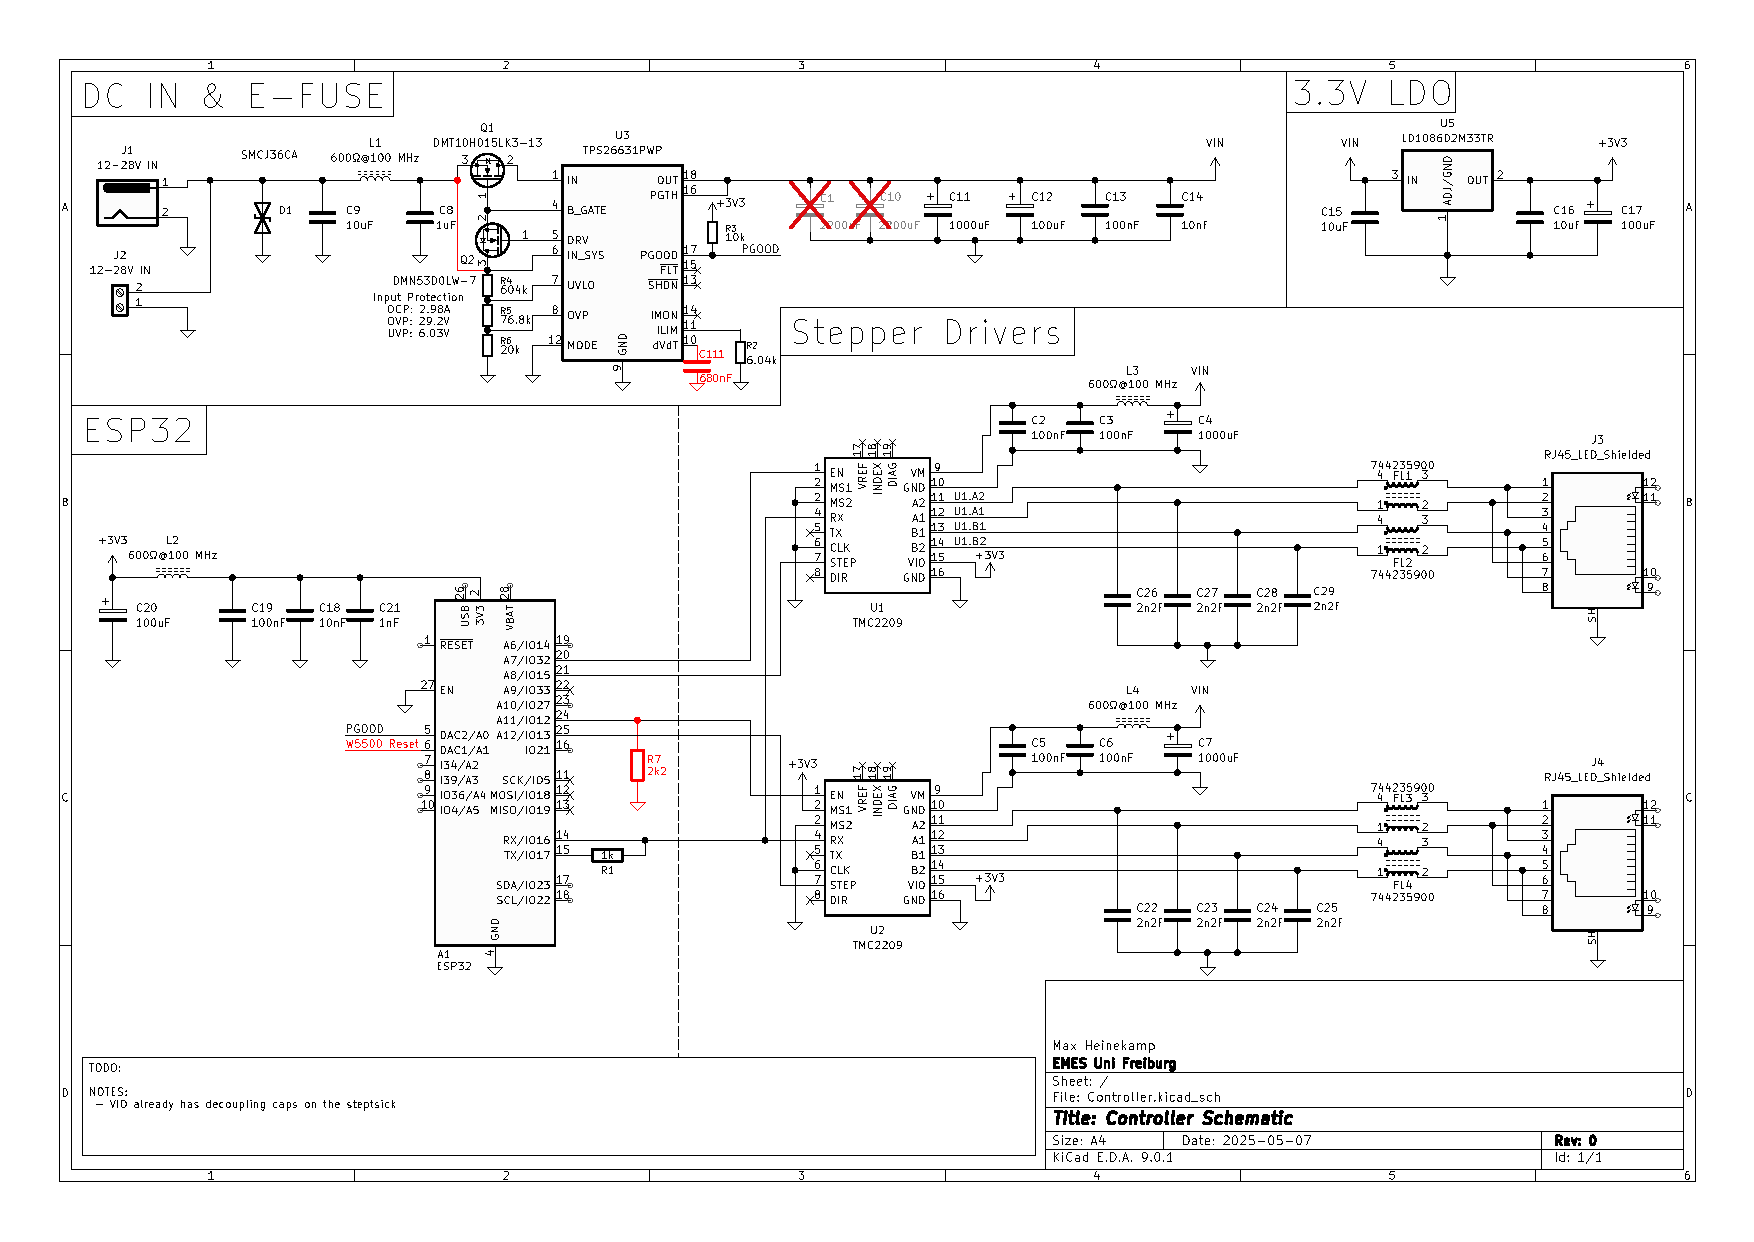
\includepdf[pages=-, landscape=true]{../Drawings/Controller-Schematic.pdf}
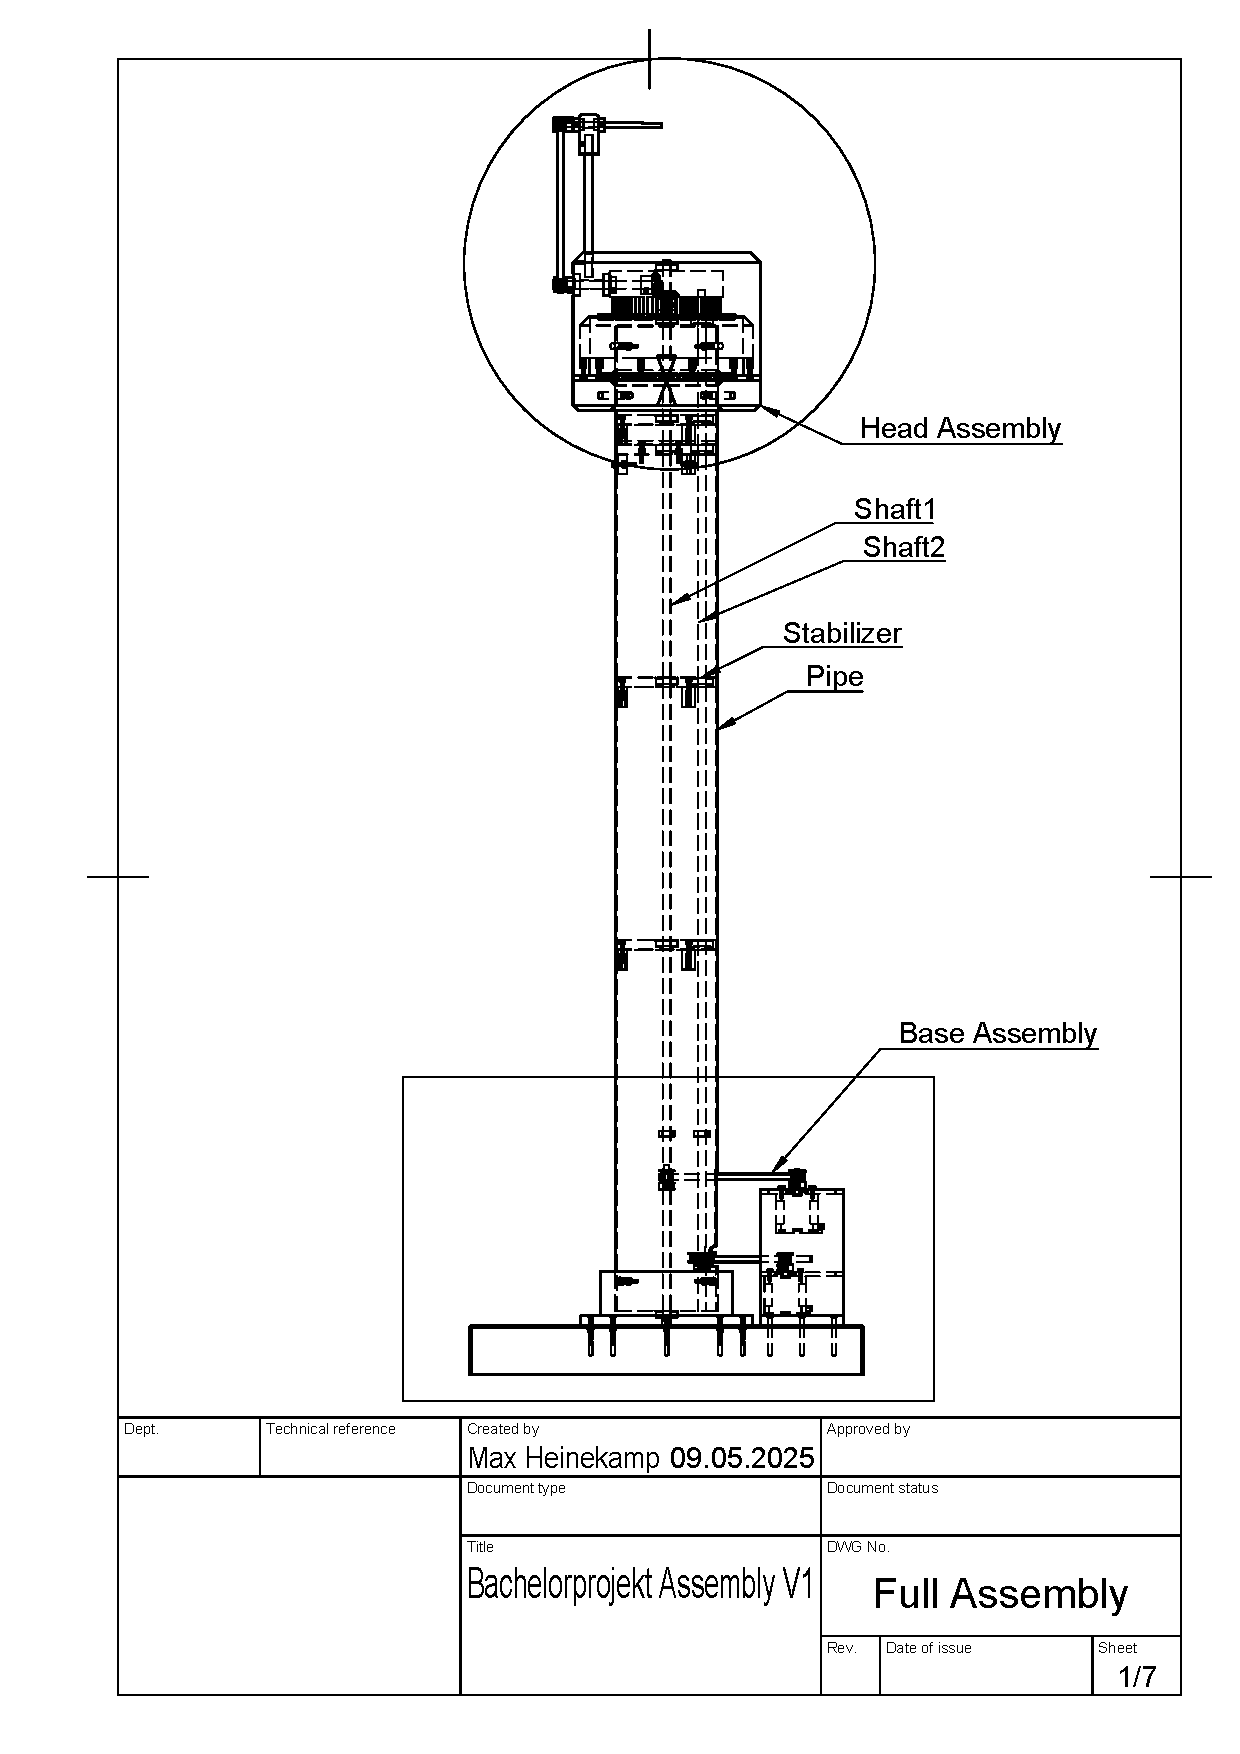
\includepdf[pages=-]{../Drawings/Mechanical-Schematic.pdf}

\section{Default values}

The following section lists the default values for the configuration parameters of the positioning system. The last column indicates whether these can be adjusted by sending the appropriate SCPI commands, as described in Section \ref{sec:command_reference}. These values are all stored in flash memory and will persist after a reboot, they can be restored by sending the \texttt{SYSTem:PRESet} command. To adjust the other parameters, modifications to the configuration file in the source code are required. 

\begin{table}[h!]
  \centering
  \begin{tabularx}{\textwidth}{|C|C|X|C|}
  \hline
  \textbf{Parameter Name} & \textbf{Default Value} & \textbf{Description} & \textbf{Configurable over SCPI} \\ \hline
  SCPI-PORT               & 5025                   & Port number for SCPI communication. & Yes \\ \hline
  IP-ADDRESS              & 192.168.0.55           & IP address for the Ethernet interface. & Yes \\ \hline
  MAC-ADDRESS             & \{0xDE, 0xAD, 0xBE, 0xEF, 0xFE, 0xED\} & MAC address for the Ethernet interface. & Yes \\ \hline
  STEPS-PER-REV           & 200                    & Number of steps per revolution for the stepper motors. & No \\ \hline
  MOTOR1-STEP-PIN         & 15                     & GPIO pin for the step signal of motor 1. & No \\ \hline
  MOTOR2-STEP-PIN         & 13                     & GPIO pin for the step signal of motor 2. & No \\ \hline
  R-SENSE                 & 0.11                   & Sense resistor value for the stepper motor drivers. & No \\ \hline
  STEP-DELAY              & 4                      & Delay between steps in milliseconds. & No \\ \hline
  RMS-CURRENT             & 1600                  & RMS current for the stepper motors in milliamps. & Yes \\ \hline
  HOLD-CURRENT            & 8                      & Hold current as a fraction (1/32) of RMS current. & Yes \\ \hline
  MICROSTEPS              & 16                     & Number of microsteps per step for the stepper motors. & Yes \\ \hline
  STEPPER1-ADDRESS        & 0                      & UART address for stepper motor 1. & No \\ \hline
  STEPPER2-ADDRESS        & 1                      & UART address for stepper motor 2. & No \\ \hline
  AXIS1-GEAR-RATIO        & 1                      & Gear ratio for axis 1. & No \\ \hline
  AXIS2-GEAR-RATIO        & 6                      & Gear ratio for axis 2. & No \\ \hline
  SPEED                   & 1000                   & Default speed for the stepper motors in steps per second. & Yes \\ \hline
  ACCELE-RATION            & 5000                   & Default acceleration for the stepper motors in steps per second squared. & Yes \\ \hline
  \end{tabularx}
  \caption{Configuration Parameters and SCPI Update Availability}
  \label{tab:config_parameters}
  \end{table}